%DIF LATEXDIFF DIFFERENCE FILE


\documentclass[12pt]{article}
 
\usepackage[margin=1in]{geometry} 
\usepackage{amsmath,amsthm,amssymb,scrextend}
\usepackage{fancyhdr}
\pagestyle{fancy}

\newcommand{\cont}{\subseteq}
\usepackage{tikz}
\usepackage{pgfplots}
\usepackage{amsmath}
\usepackage[mathscr]{euscript}
\let\euscr\mathscr \let\mathscr\relax% just so we can load this and rsfs
\usepackage[scr]{rsfso}
\usepackage{amsthm}
\usepackage{amssymb}
\usepackage{multicol}
\usepackage[colorlinks=true, pdfstartview=FitV, linkcolor=blue,
citecolor=blue, urlcolor=blue]{hyperref}

\usepackage{parskip}
\usepackage{graphicx}
\usepackage{subcaption}
\usepackage{booktabs}
\usepackage{ulem}

%DIF PREAMBLE EXTENSION ADDED BY LATEXDIFF
%DIF UNDERLINE PREAMBLE %DIF PREAMBLE
\RequirePackage[normalem]{ulem} %DIF PREAMBLE
\RequirePackage{color}\definecolor{RED}{rgb}{1,0,0}\definecolor{BLUE}{rgb}{0,0,1} %DIF PREAMBLE
\providecommand{\DIFaddtex}[1]{{\protect\color{blue}\uwave{#1}}} %DIF PREAMBLE
\providecommand{\DIFdeltex}[1]{{\protect\color{red}\sout{#1}}}                      %DIF PREAMBLE
%DIF SAFE PREAMBLE %DIF PREAMBLE
\providecommand{\DIFaddbegin}{} %DIF PREAMBLE
\providecommand{\DIFaddend}{} %DIF PREAMBLE
\providecommand{\DIFdelbegin}{} %DIF PREAMBLE
\providecommand{\DIFdelend}{} %DIF PREAMBLE
\providecommand{\DIFmodbegin}{} %DIF PREAMBLE
\providecommand{\DIFmodend}{} %DIF PREAMBLE
%DIF FLOATSAFE PREAMBLE %DIF PREAMBLE
\providecommand{\DIFaddFL}[1]{\DIFadd{#1}} %DIF PREAMBLE
\providecommand{\DIFdelFL}[1]{\DIFdel{#1}} %DIF PREAMBLE
\providecommand{\DIFaddbeginFL}{} %DIF PREAMBLE
\providecommand{\DIFaddendFL}{} %DIF PREAMBLE
\providecommand{\DIFdelbeginFL}{} %DIF PREAMBLE
\providecommand{\DIFdelendFL}{} %DIF PREAMBLE
%DIF HYPERREF PREAMBLE %DIF PREAMBLE
\providecommand{\DIFadd}[1]{\texorpdfstring{\DIFaddtex{#1}}{#1}} %DIF PREAMBLE
\providecommand{\DIFdel}[1]{\texorpdfstring{\DIFdeltex{#1}}{}} %DIF PREAMBLE
\newcommand{\DIFscaledelfig}{0.5}
%DIF HIGHLIGHTGRAPHICS PREAMBLE %DIF PREAMBLE
\RequirePackage{settobox} %DIF PREAMBLE
\RequirePackage{letltxmacro} %DIF PREAMBLE
\newsavebox{\DIFdelgraphicsbox} %DIF PREAMBLE
\newlength{\DIFdelgraphicswidth} %DIF PREAMBLE
\newlength{\DIFdelgraphicsheight} %DIF PREAMBLE
% store original definition of \includegraphics %DIF PREAMBLE
\LetLtxMacro{\DIFOincludegraphics}{\includegraphics} %DIF PREAMBLE
\newcommand{\DIFaddincludegraphics}[2][]{{\color{blue}\fbox{\DIFOincludegraphics[#1]{#2}}}} %DIF PREAMBLE
\newcommand{\DIFdelincludegraphics}[2][]{% %DIF PREAMBLE
\sbox{\DIFdelgraphicsbox}{\DIFOincludegraphics[#1]{#2}}% %DIF PREAMBLE
\settoboxwidth{\DIFdelgraphicswidth}{\DIFdelgraphicsbox} %DIF PREAMBLE
\settoboxtotalheight{\DIFdelgraphicsheight}{\DIFdelgraphicsbox} %DIF PREAMBLE
\scalebox{\DIFscaledelfig}{% %DIF PREAMBLE
\parbox[b]{\DIFdelgraphicswidth}{\usebox{\DIFdelgraphicsbox}\\[-\baselineskip] \rule{\DIFdelgraphicswidth}{0em}}\llap{\resizebox{\DIFdelgraphicswidth}{\DIFdelgraphicsheight}{% %DIF PREAMBLE
\setlength{\unitlength}{\DIFdelgraphicswidth}% %DIF PREAMBLE
\begin{picture}(1,1)% %DIF PREAMBLE
\thicklines\linethickness{2pt} %DIF PREAMBLE
{\color[rgb]{1,0,0}\put(0,0){\framebox(1,1){}}}% %DIF PREAMBLE
{\color[rgb]{1,0,0}\put(0,0){\line( 1,1){1}}}% %DIF PREAMBLE
{\color[rgb]{1,0,0}\put(0,1){\line(1,-1){1}}}% %DIF PREAMBLE
\end{picture}% %DIF PREAMBLE
}\hspace*{3pt}}} %DIF PREAMBLE
} %DIF PREAMBLE
\LetLtxMacro{\DIFOaddbegin}{\DIFaddbegin} %DIF PREAMBLE
\LetLtxMacro{\DIFOaddend}{\DIFaddend} %DIF PREAMBLE
\LetLtxMacro{\DIFOdelbegin}{\DIFdelbegin} %DIF PREAMBLE
\LetLtxMacro{\DIFOdelend}{\DIFdelend} %DIF PREAMBLE
\DeclareRobustCommand{\DIFaddbegin}{\DIFOaddbegin \let\includegraphics\DIFaddincludegraphics} %DIF PREAMBLE
\DeclareRobustCommand{\DIFaddend}{\DIFOaddend \let\includegraphics\DIFOincludegraphics} %DIF PREAMBLE
\DeclareRobustCommand{\DIFdelbegin}{\DIFOdelbegin \let\includegraphics\DIFdelincludegraphics} %DIF PREAMBLE
\DeclareRobustCommand{\DIFdelend}{\DIFOaddend \let\includegraphics\DIFOincludegraphics} %DIF PREAMBLE
\LetLtxMacro{\DIFOaddbeginFL}{\DIFaddbeginFL} %DIF PREAMBLE
\LetLtxMacro{\DIFOaddendFL}{\DIFaddendFL} %DIF PREAMBLE
\LetLtxMacro{\DIFOdelbeginFL}{\DIFdelbeginFL} %DIF PREAMBLE
\LetLtxMacro{\DIFOdelendFL}{\DIFdelendFL} %DIF PREAMBLE
\DeclareRobustCommand{\DIFaddbeginFL}{\DIFOaddbeginFL \let\includegraphics\DIFaddincludegraphics} %DIF PREAMBLE
\DeclareRobustCommand{\DIFaddendFL}{\DIFOaddendFL \let\includegraphics\DIFOincludegraphics} %DIF PREAMBLE
\DeclareRobustCommand{\DIFdelbeginFL}{\DIFOdelbeginFL \let\includegraphics\DIFdelincludegraphics} %DIF PREAMBLE
\DeclareRobustCommand{\DIFdelendFL}{\DIFOaddendFL \let\includegraphics\DIFOincludegraphics} %DIF PREAMBLE
%DIF END PREAMBLE EXTENSION ADDED BY LATEXDIFF

\begin{document}

%%%%%% HEADER %%%%%%

\lhead{MLaRPiS}
\chead{Week 1}
\rhead{Giuliana Orizzonte}

%%%%%% TITLE PAGE %%%%%%

\begin{titlepage}
    \centering
    \vspace*{\stretch{1}}
    \Large\textbf{Week 1: Markup Languages}\\
    \vspace{1.5cm}
    Markup Languages and Reproducible Programming in Statistics\\
    \vspace{1cm}
    \large{Giuliana Orizzonte}\\
    \vspace{8cm}
    Methodology and Statistics for the Behavioural, Biomedical and Social Sciences\\
    \vspace{0.5cm}
    Utrecht University\\
    \vspace{\stretch{2}}
\end{titlepage}


\section{Title Page}
The first page of this document is a customized title page that includes my name alongside information about the course, the assignment, the program, and the university.

\section{Equation}
The equation $E$ defines the loss function of a multi-modal autoencoder:

\begin{equation}
E = argmin_{f,g} (\alpha Loss_1 (x_1, g_1(f_1(x_1))) + \ldots \ + \beta Loss_k (x_k, g_k(f_k(x_k))),\label{AE} 
\end{equation}

where $\alpha ,\ldots, \beta$ are weights that sum up to 1 and reflect the relative importance of each $k^{th}$ input matrix.

\section{Section}
I realize that if through science I can seize phenomena and enumerate them, I cannot, for all that, apprehend the world.

\subsection{Subsection}
Were I to trace its entire relief with my finger, I should not know any more. And you give me the choice between a description that is sure but that teaches me nothing and hypotheses that claim to teach me but that are not sure.

\section{Figures and Table}
The figures and table are on a standalone page, as per the example file.

\vspace{6cm}

\begin{figure}[t]
\centering
\begin{subfigure}{0.48\textwidth}
    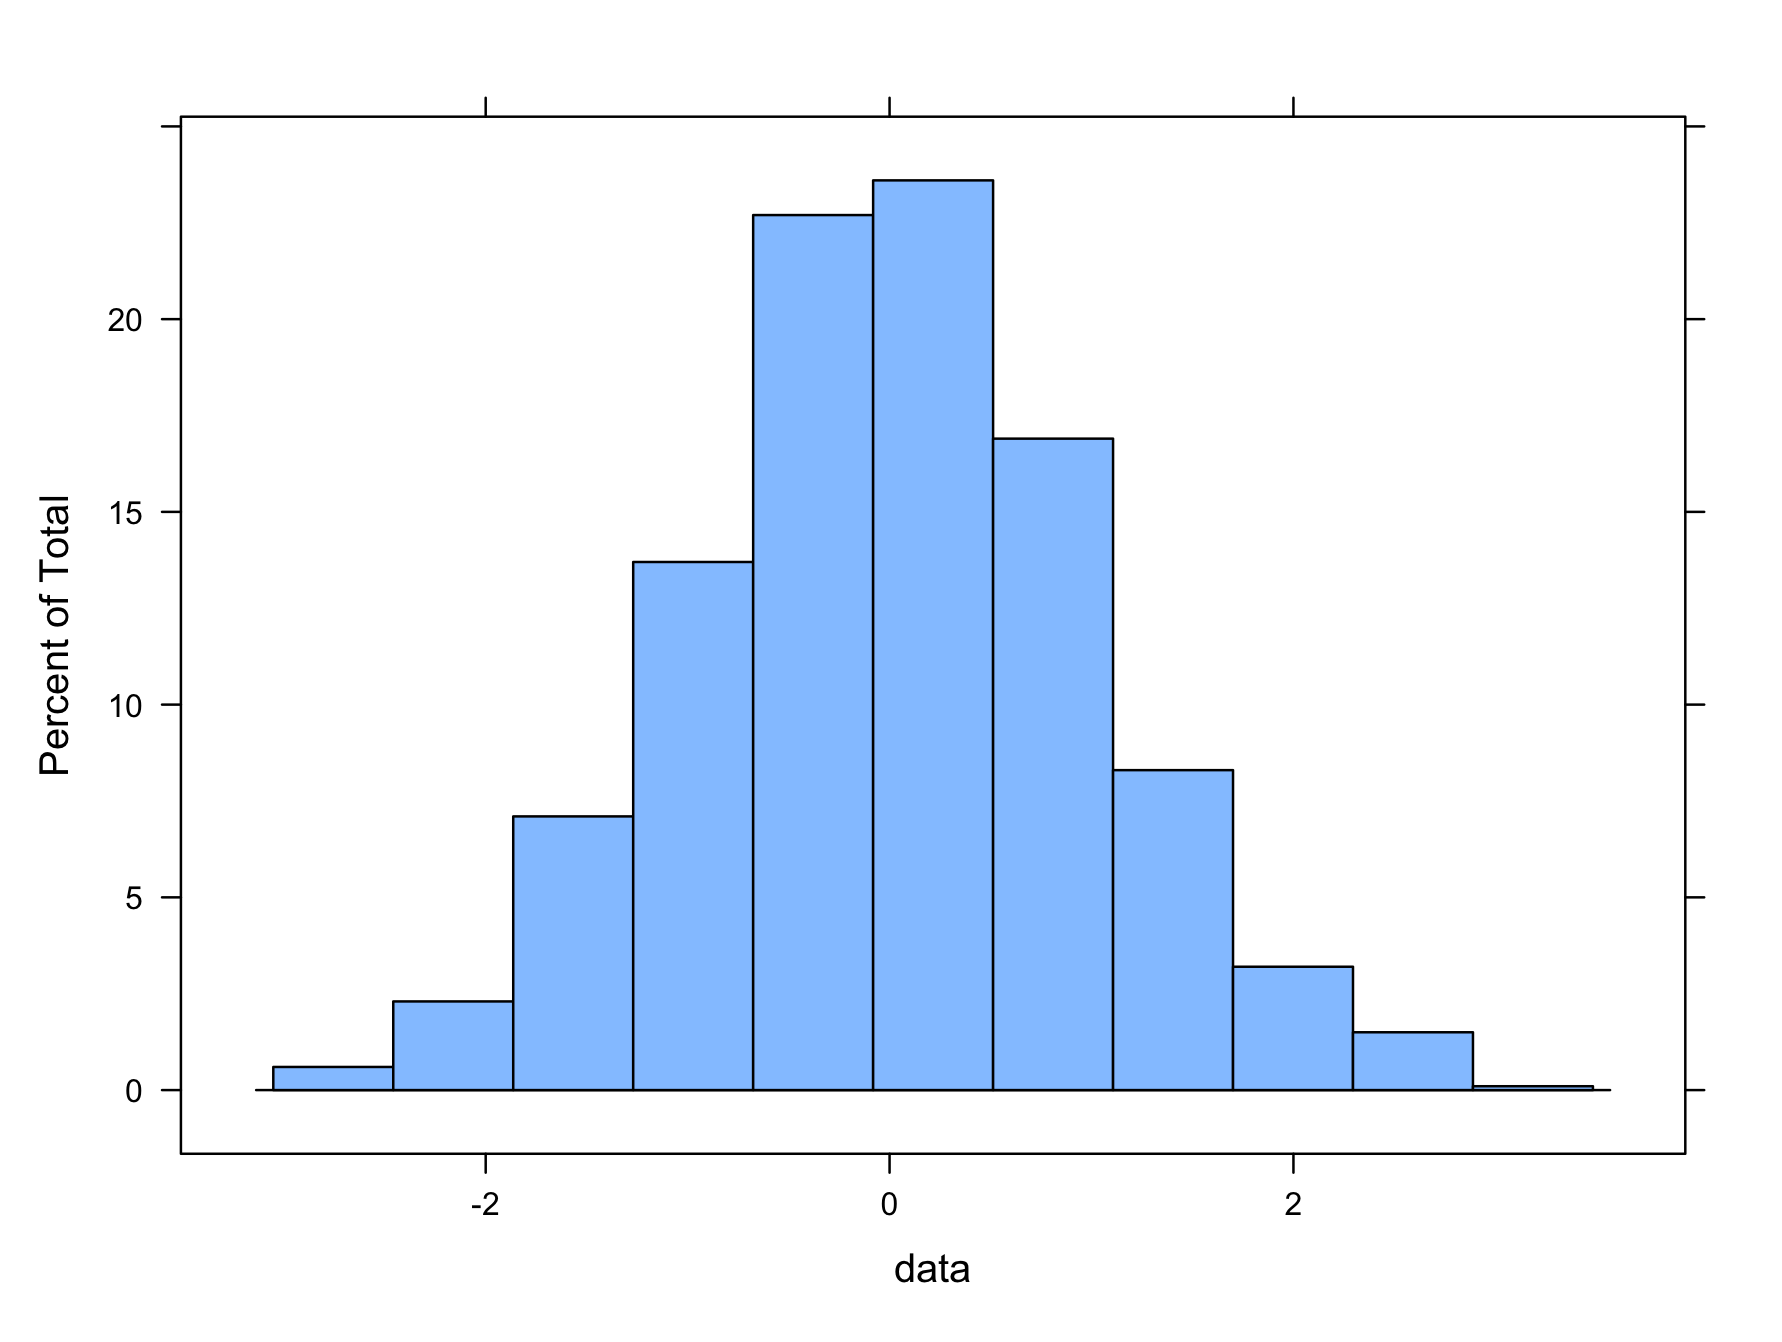
\includegraphics[width=\textwidth]{hist.jpg}
    \caption{Histogram}
    \label{histogram}
\end{subfigure}
\hfill
\begin{subfigure}{0.48\textwidth}
    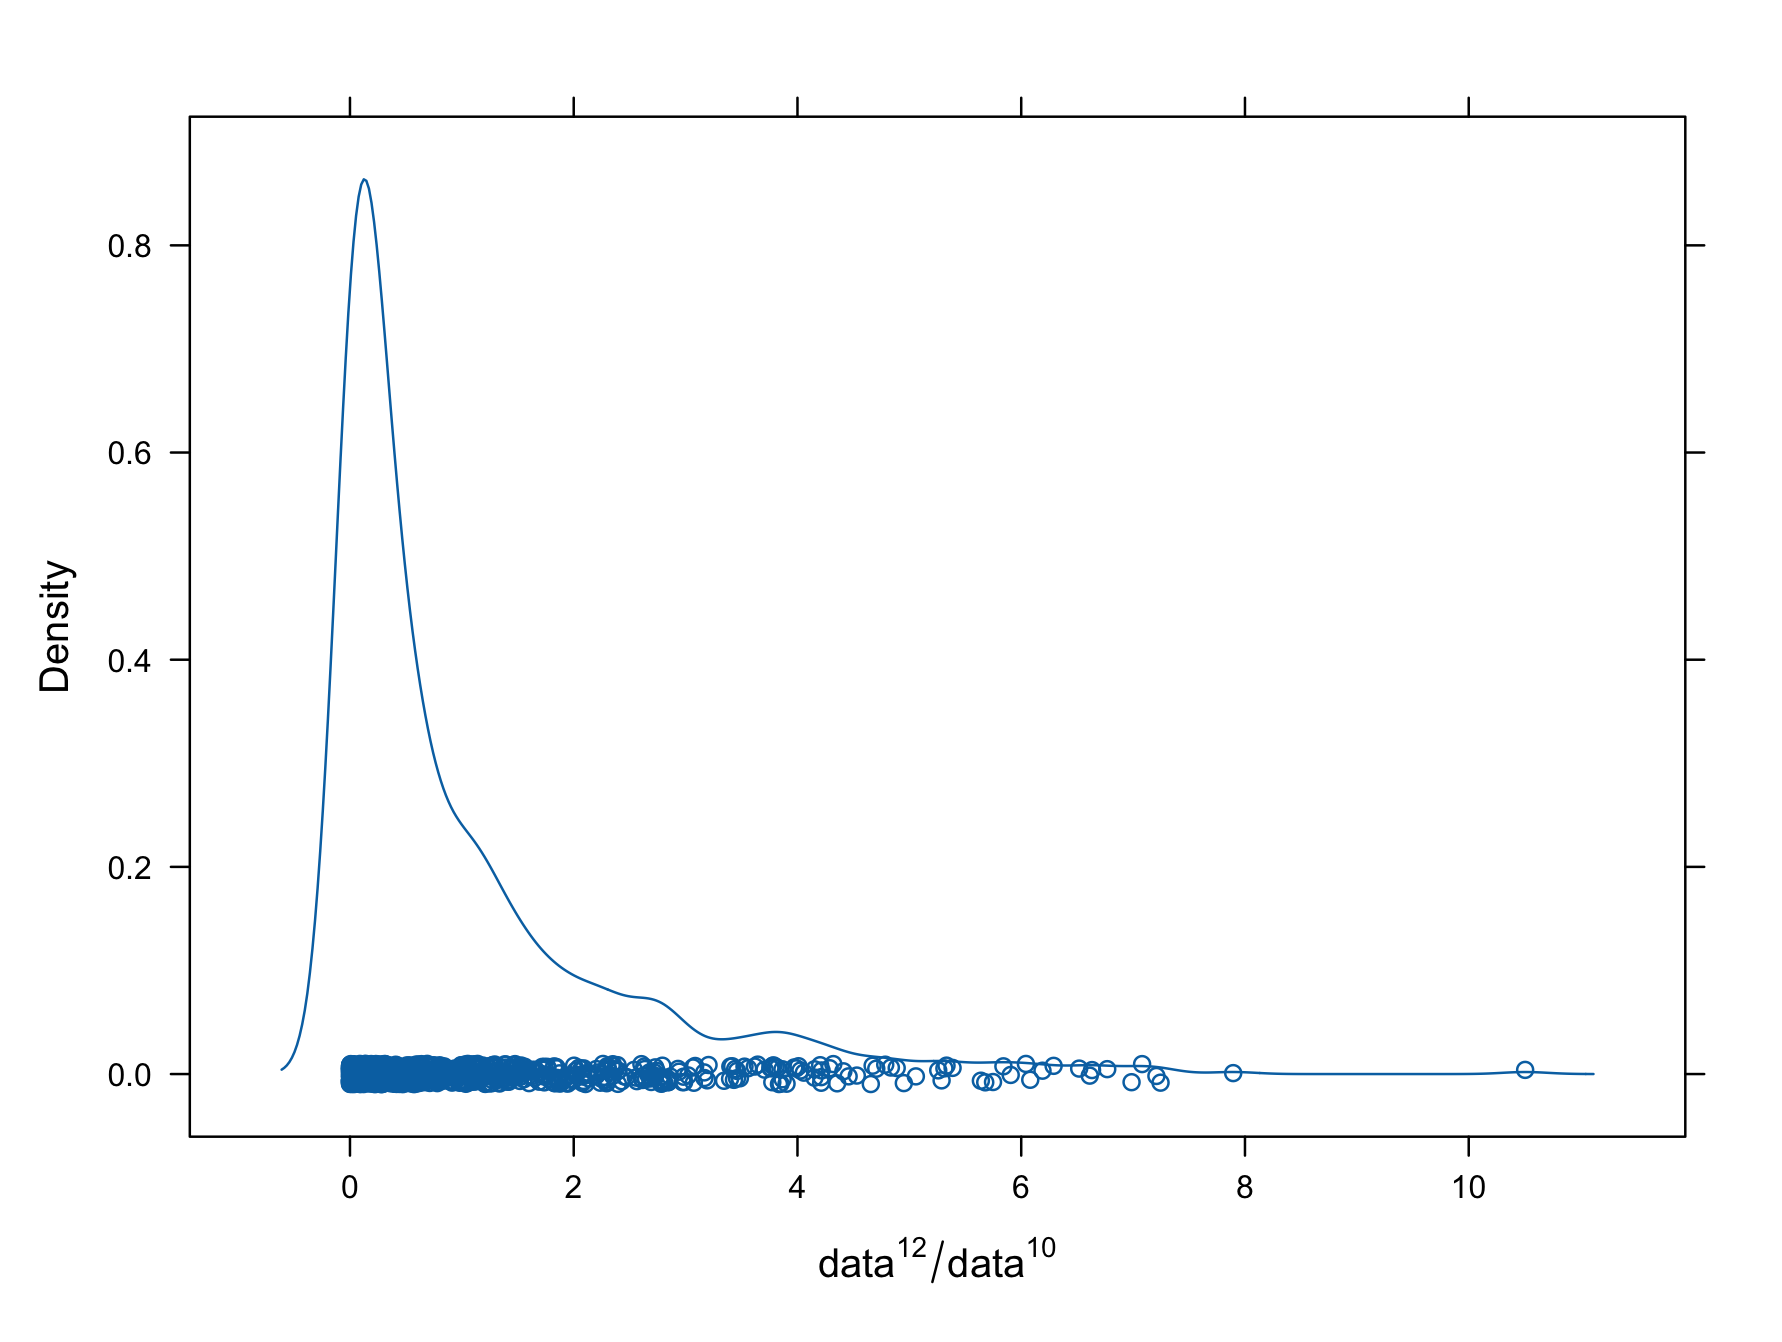
\includegraphics[width=\textwidth]{density.jpg}
    \caption{Densityplot}
    \label{density}
\end{subfigure}
\hfill
\begin{subfigure}{0.48\textwidth}
    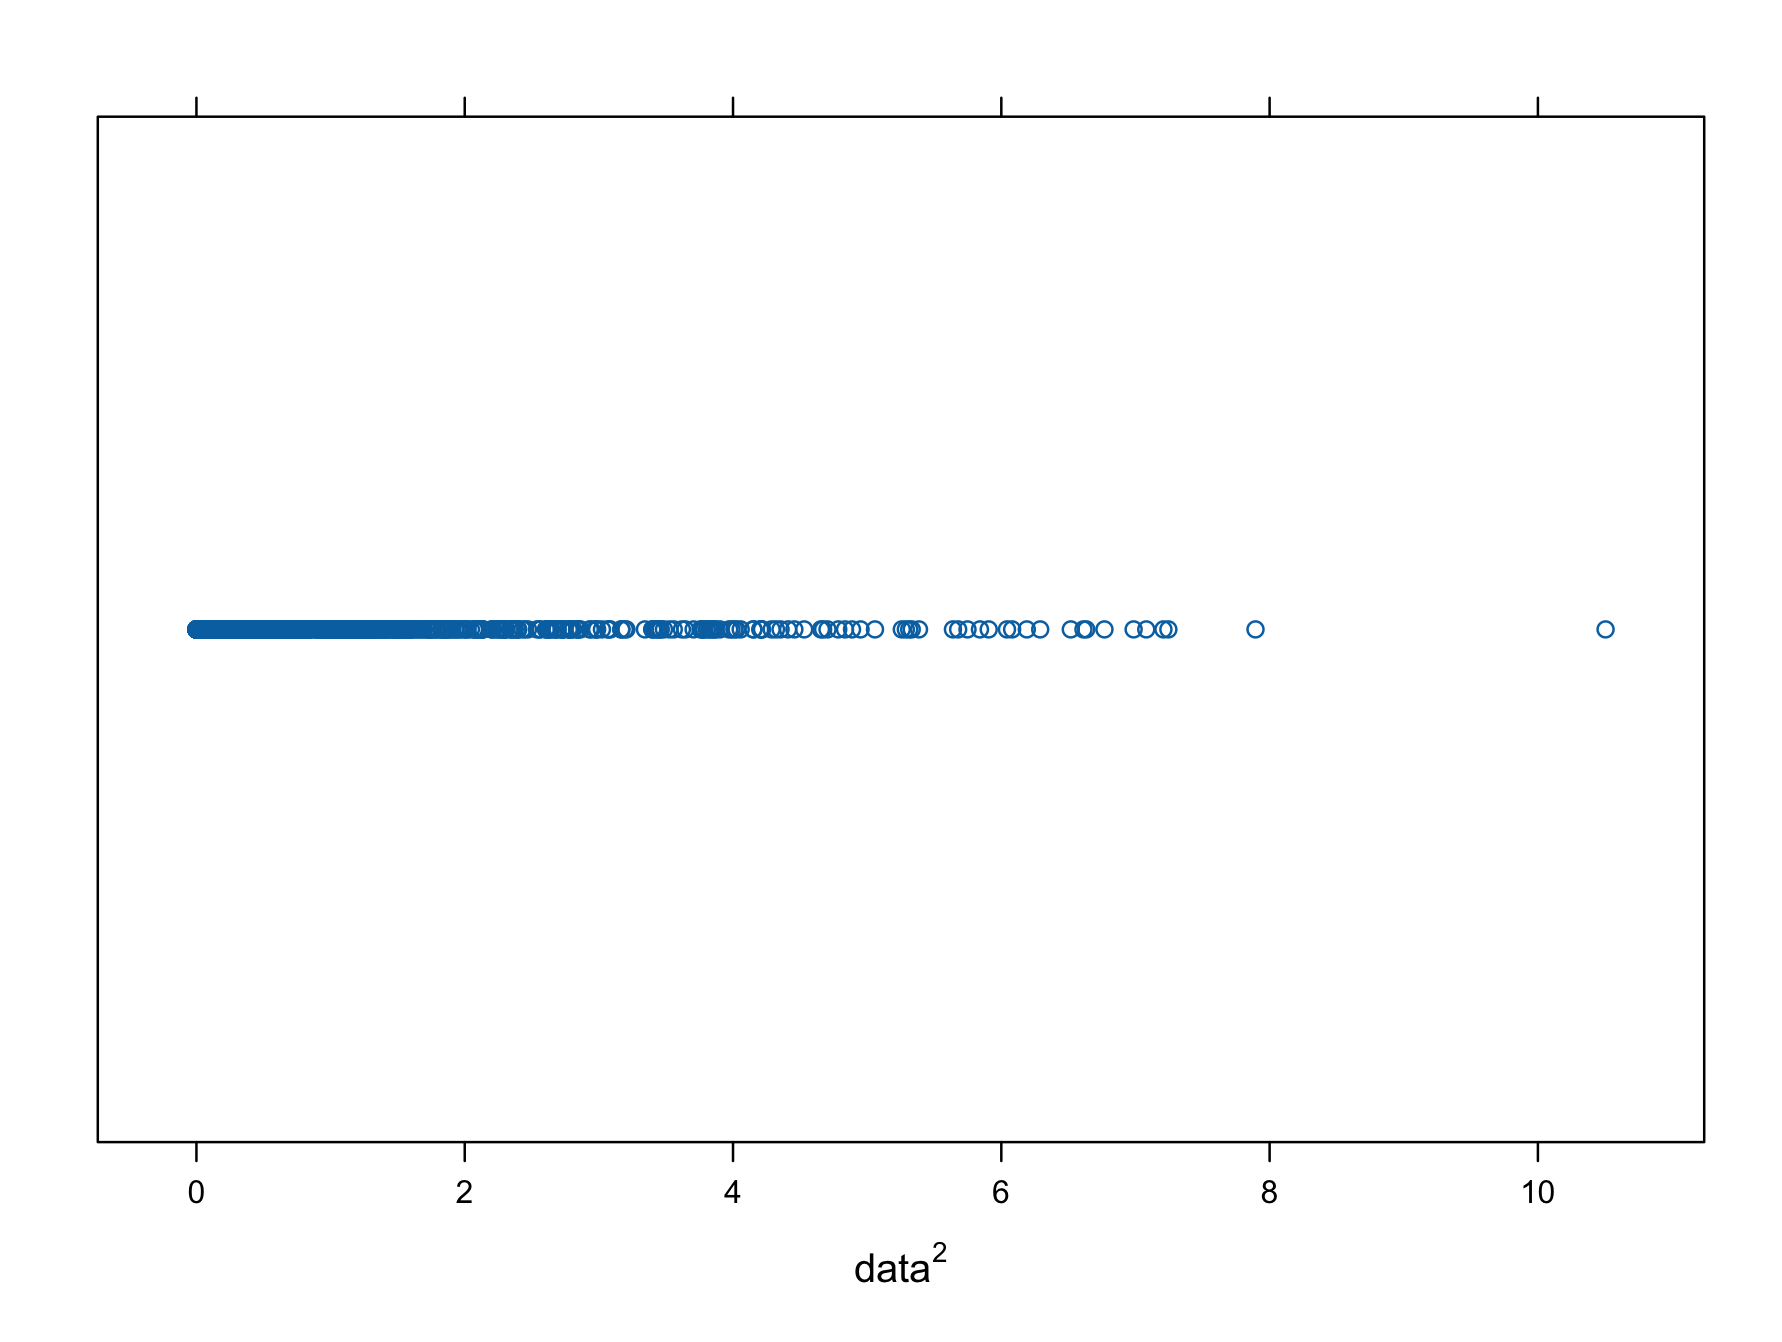
\includegraphics[width=\textwidth]{stripplot.jpg}
    \caption{Stripplot}
    \label{stripplot}
\end{subfigure}
\hfill
\begin{subfigure}{0.48\textwidth}
    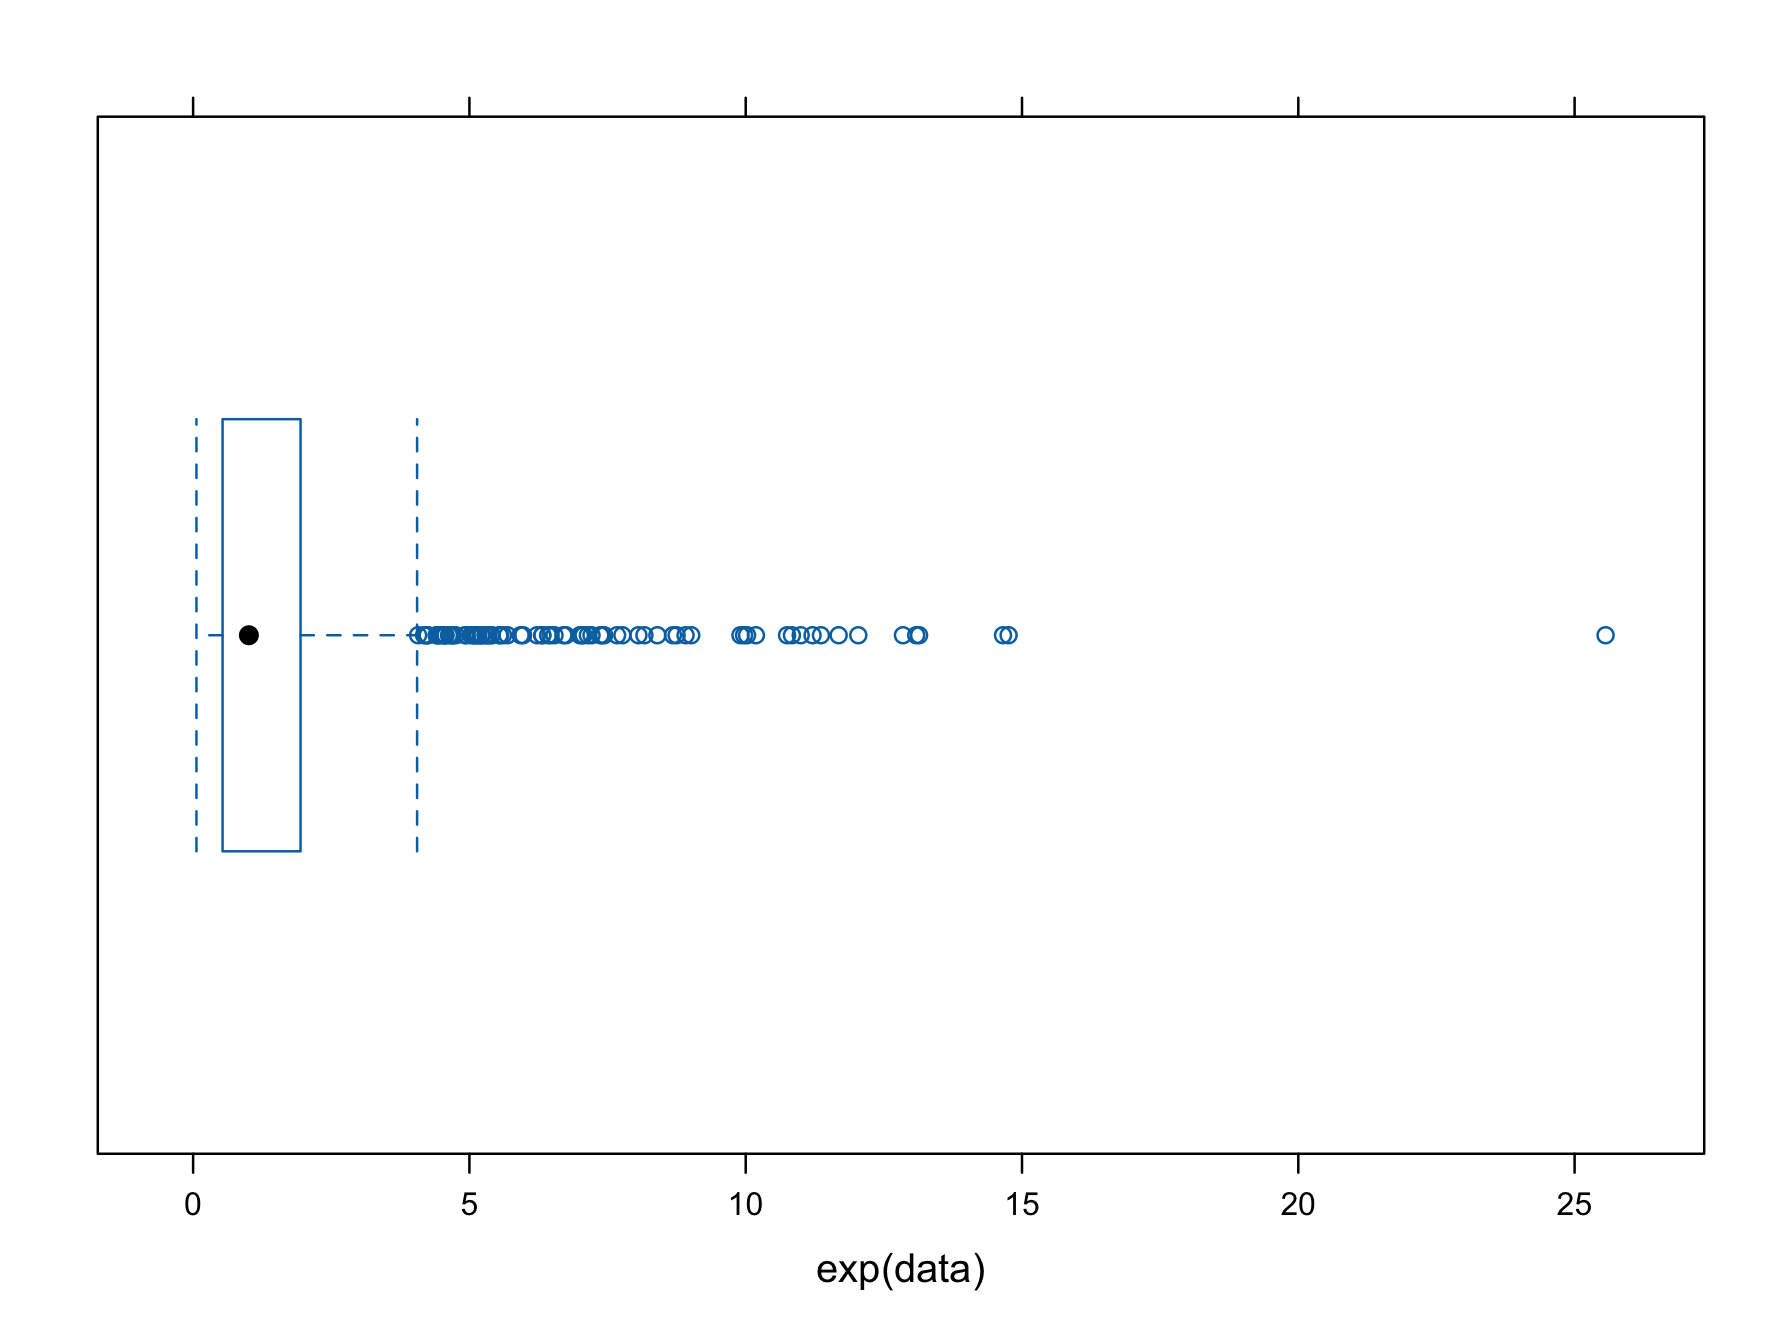
\includegraphics[width=\textwidth]{boxplot.jpg}
    \caption{Boxplot}
    \label{boxplot}
\end{subfigure}

\caption{Different plots of the same data, sometimes transformed. No particular objective other than it being an exercise.}
\label{fig:figures}
\end{figure}

\begin{table}[!hb]
\centering
\caption{The same data, but now in a table. Only the first nine rows are displayed.}
\begin{tabular}{@{}ccccc@{}}
\toprule
  & data & squared1 & squared2 & exponent \\ \midrule
1 & -0.56 & 0.31 & 0.31 & 0.57 \\
2 & -0.23 & 0.05 & 0.05 & 0.79 \\
3 & 1.56 & 2.43 & 2.43 & 4.75 \\
4 & 0.07 & 0.00 & 0.00 & 1.07 \\
5 & 0.13 & 0.02 & 0.02 & 1.14 \\
6 & 1.72 & 2.94 & 2.94 & 5.56 \\
7 & 0.46 & 0.21 & 0.21 & 1.59 \\
8 & -1.27 & 1.60 & 1.60 & 0.28 \\
9 & -0.69 & 0.47 & 0.47 & 0.50 \\ \bottomrule
\end{tabular}
\end{table}

\section{Fairytale}

\textit{The Enchanted Garden and the \DIFdelbegin \DIFdel{Luminous }\DIFdelend \DIFaddbegin \DIFadd{Magical }\DIFaddend Dove}

Once, in a land covered by mists and whispers, there lay an enchanting garden hidden behind a great stone wall. No one knew who had built the wall or why, but one thing was for certain – nobody had ever seen what was behind it.

A little \DIFdelbegin \DIFdel{girl named Clara }\DIFdelend \DIFaddbegin \DIFadd{boy named Peter }\DIFaddend lived in a village nearby. \DIFdelbegin \DIFdel{Fueled }\DIFdelend \DIFaddbegin \DIFadd{Fuelled }\DIFaddend by curiosity and tales of magical creatures, \DIFdelbegin \DIFdel{she }\DIFdelend \DIFaddbegin \DIFadd{he }\DIFaddend often dreamt of the wonders that the walled garden might hold. One day, unable to resist its lure any longer, \DIFdelbegin \DIFdel{she }\DIFdelend \DIFaddbegin \DIFadd{he }\DIFaddend decided to find a way in.

As \DIFdelbegin \DIFdel{she }\DIFdelend \DIFaddbegin \DIFadd{he }\DIFaddend approached the towering stone barrier, \DIFdelbegin \DIFdel{she }\DIFdelend \DIFaddbegin \DIFadd{he }\DIFaddend noticed a tiny gap just big enough for \DIFdelbegin \DIFdel{her }\DIFdelend \DIFaddbegin \DIFadd{him }\DIFaddend to peek through. The garden inside was bathed in a shimmering golden light, unlike any \DIFdelbegin \DIFdel{she }\DIFdelend \DIFaddbegin \DIFadd{he }\DIFaddend had ever seen. To \DIFdelbegin \DIFdel{her }\DIFdelend \DIFaddbegin \DIFadd{his }\DIFaddend amazement, in the center stood a magnificent tree with leaves that glittered as if they were made of starlight. And resting on one of its branches was a dove, glowing with the same luminous hue.

Before \DIFdelbegin \DIFdel{she }\DIFdelend \DIFaddbegin \DIFadd{he }\DIFaddend could process this beautiful sight, the dove spoke to \DIFdelbegin \DIFdel{her }\DIFdelend \DIFaddbegin \DIFadd{his }\DIFaddend in a voice as soft as the wind, "To enter the garden, one must share a pure and selfless desire."

\DIFdelbegin \DIFdel{Clara, with her }\DIFdelend \DIFaddbegin \DIFadd{Peter, with his }\DIFaddend heart pounding, whispered \DIFdelbegin \DIFdel{her }\DIFdelend \DIFaddbegin \DIFadd{his }\DIFaddend wish, "I wish for everyone in my village to be happy and free from suffering."

The massive stone door, seemingly of its own accord, began to open. The luminous dove flew to \DIFdelbegin \DIFdel{Clara }\DIFdelend \DIFaddbegin \DIFadd{Peter }\DIFaddend and rested on \DIFdelbegin \DIFdel{her }\DIFdelend \DIFaddbegin \DIFadd{his }\DIFaddend shoulder. "Your wish is genuine, and so you may enter," it said.

Inside, the garden was more wondrous than \DIFdelbegin \DIFdel{Clara }\DIFdelend \DIFaddbegin \DIFadd{Peter }\DIFaddend had ever imagined. Flowers sang in soft harmonies, and a gentle breeze carried the sweetest of fragrances. Every step \DIFdelbegin \DIFdel{she }\DIFdelend \DIFaddbegin \DIFadd{he }\DIFaddend took made the grass shimmer with colors she'd never seen before.

The dove explained that this was an Enchanted Garden, a place where one’s purest wishes could come true. But, there was a catch. To make \DIFdelbegin \DIFdel{her }\DIFdelend \DIFaddbegin \DIFadd{his }\DIFaddend wish a reality, \DIFdelbegin \DIFdel{Clara }\DIFdelend \DIFaddbegin \DIFadd{Peter }\DIFaddend had to plant a seed from the magical tree in \DIFdelbegin \DIFdel{her }\DIFdelend \DIFaddbegin \DIFadd{his }\DIFaddend village and care for it with unwavering love and dedication.

\DIFdelbegin \DIFdel{Clara }\DIFdelend \DIFaddbegin \DIFadd{Peter }\DIFaddend accepted the challenge. With the seed safely tucked in \DIFdelbegin \DIFdel{her }\DIFdelend \DIFaddbegin \DIFadd{his }\DIFaddend pocket and the dove guiding her, \DIFdelbegin \DIFdel{she returned to her }\DIFdelend \DIFaddbegin \DIFadd{he returned to his }\DIFaddend village.

Years went by, and with \DIFdelbegin \DIFdel{Clara}\DIFdelend \DIFaddbegin \DIFadd{Peter}\DIFaddend 's love, the seed grew into a magnificent tree, similar to the one in the Enchanted Garden. With its growth, joy and happiness blossomed in the village like never before.

\DIFdelbegin \DIFdel{Clara's selfless wish not only transformed her village but also changed her. She became known as the Keeper of Joy, teaching future generations about love, compassion, and the magic of selfless wishes.
}%DIFDELCMD < 

%DIFDELCMD < %%%
\DIFdelend And so, in a village once shadowed by mystery, there stood a tree that bore witness to the pure heart of a \DIFdelbegin \DIFdel{girl and her }\DIFdelend \DIFaddbegin \DIFadd{boy and his }\DIFaddend luminous companion, reminding everyone that magic was always just a wish away.

\end{document}